\chapter{DevOps}
\label{chapter:mant}

Una vez hemos llegado a esta parte del documento, ya hemos realizado el análisis completo de los datos y hemos dejado el modelo en un entorno productivo clasificando llamadas en \textit{real-time}; sin embargo sería muy atrevido dar el proyecto por finalizado.

Probablemente surgirán nuevos datos, dispondremos de nuevas etiquetas, nuestro \textit{software} se degradará, crearemos nuevos y mejores modelos con ideas más o menos brillantes, etc. Este universo cambiante provocará que se modifiquen y/o se creen nuevos \textit{software} y modelos con bastante frecuencia y será necesario llevar de nuevo a producción.  

Este capítulo tiene como objetivo definir los mecanismos y la metodología que hemos establecido para poder reaccionar con gran agilidad ante el cambio, algo esencial hoy en día. En la sección \ref{section:mant:devops} haremos una introducción a la metodología DevOps que acuñaremos en nuestro proyecto, posteriormente pondremos foco en algunos aspectos importantes: La degradación del modelo (sección \ref{section:mant:efi}) y la integración y el despliegue continuos (sección \ref{section:mant:cicd}).


\section{Introducción DevOps}

\textit{DevOps} es una metodología de desarrollo de \textit{software} que se centra en la comunicación entre las áreas de desarrollo y las áreas de producción. El objetivo principal de \textit{DevOps} es reducir el \textit{time to marquet} a la vez que mejorar la calidad del \textit{software}.

\label{section:mant:devops}


\begin{figure}[!ht]
	\centering
	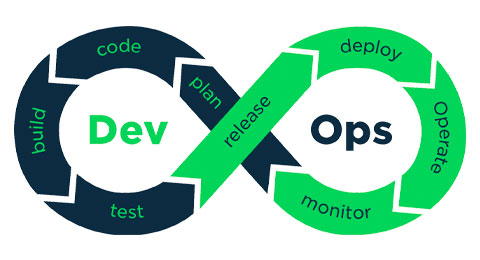
\includegraphics[width=0.7\textwidth]{images/mant/devops}
	\caption{Metodología DevOps. Fuente \cite{devops}}
	\label{fig:devops}
\end{figure}




En la figura \ref{fig:devops} podemos ver las ocho fases de un flujo DevOps que describiremos brevemente: 

\begin{itemize}
\item \textbf{Planificar}:  En esta fase se definen las tareas que se van a realizar a lo largo de las siguientes fases. 

\item \textbf{Codificar}: Es la fase en la que se implementa el nuevo \textit{software}.

\item \textbf{Construir}: La fases anteriores no han aportado nada nuevo respecto al desarrollo de \textit{software} tradicional. En esta fase se procede al compilado del código que normalmente es iniciado por algún automatismo al realizar un \textit{push} al repositorio de control de versiones.

\item \textbf{Probar}: Una vez se ha compilado el \textit{software} lo ideal es realizar pruebas sobre el mismo en un entorno de pruebas para garantizar su  funcionamiento.

\item \textbf{Versionar}: Es el punto en el que decimos que una compilación está lista para implantarse en producción. 

\item \textbf{Despliegue}: En el momento que tenemos una versión lista para el entorno de producción pasamos a realizar el despliegue en el entorno productivo.

\item \textbf{Operación}: Llegados a este punto la nueva versión ya esta en producción. Es esencial en esta parte recoger \textit{feedback} del funcionamiento de la versión desplegada.

\item \textbf{Monitorización}: Por último, pero no menos importante, debemos poner foco en la monitorización que nos sirva junto con el \textit{feedback} de la fase anterior para la fase de planificación.


 \end{itemize}


Tras ver las fases del flujo DevOps es fácil identificar las posibilidades de integración continua, entrega continua, despliegue continuo y \textit{feedback} continuo que normalmente escuchamos. Este ``todo'' continuo se debe a que la continuidad es el núcleo de todo proyecto 

Si bien, al tratarse de un proyecto individual y con un único entorno, no ha sido posible cubrir todas las etapas de la metodología, sí que se han provisto las herramientas necesarias para su implantación definitiva. 

En nuestro caso hemos ayudado a crear un flujo DevOps dando los siguientes pasos: 

\begin{itemize}
\item\textbf{ Automatizando el proceso de compilación y de pruebas unitarias}  del software desarrollado.
\item Realizando \textbf{despliegues automáticos} del software una vez validado.
\item Poniendo foco constante en la \textbf{monitorización}.
\end{itemize}


\section{Degradación del modelo/ \textit{Feedback} continuo}
\label{section:mant:efi}
Aunque el \textit{software} desarrollado también es propenso a degradarse con el paso del tiempo, si hay algo que tenemos seguro que se va a degradar en este universo cambiante, es el modelo. Nuestro modelo se alimenta con las transcripciones de los clientes que están basadas en el servicio que ofrecemos en cada momento, en las inquietudes de nuestros clientes y otros muchos factores externos que pueden influir en la temática de las conversaciones que recibimos.

La certeza en la degradación de nuestro modelo hace que tengamos que monitorizar constantemente el rendimiento del mismo, en el caso del modelo supervisado que hemos llevado a producción, nos lleva a seguir testándolo constantemente introduciendo en el flujo llamadas de control etiquetadas para medir su eficiencia.  




\begin{figure}[!ht]
	\centering
	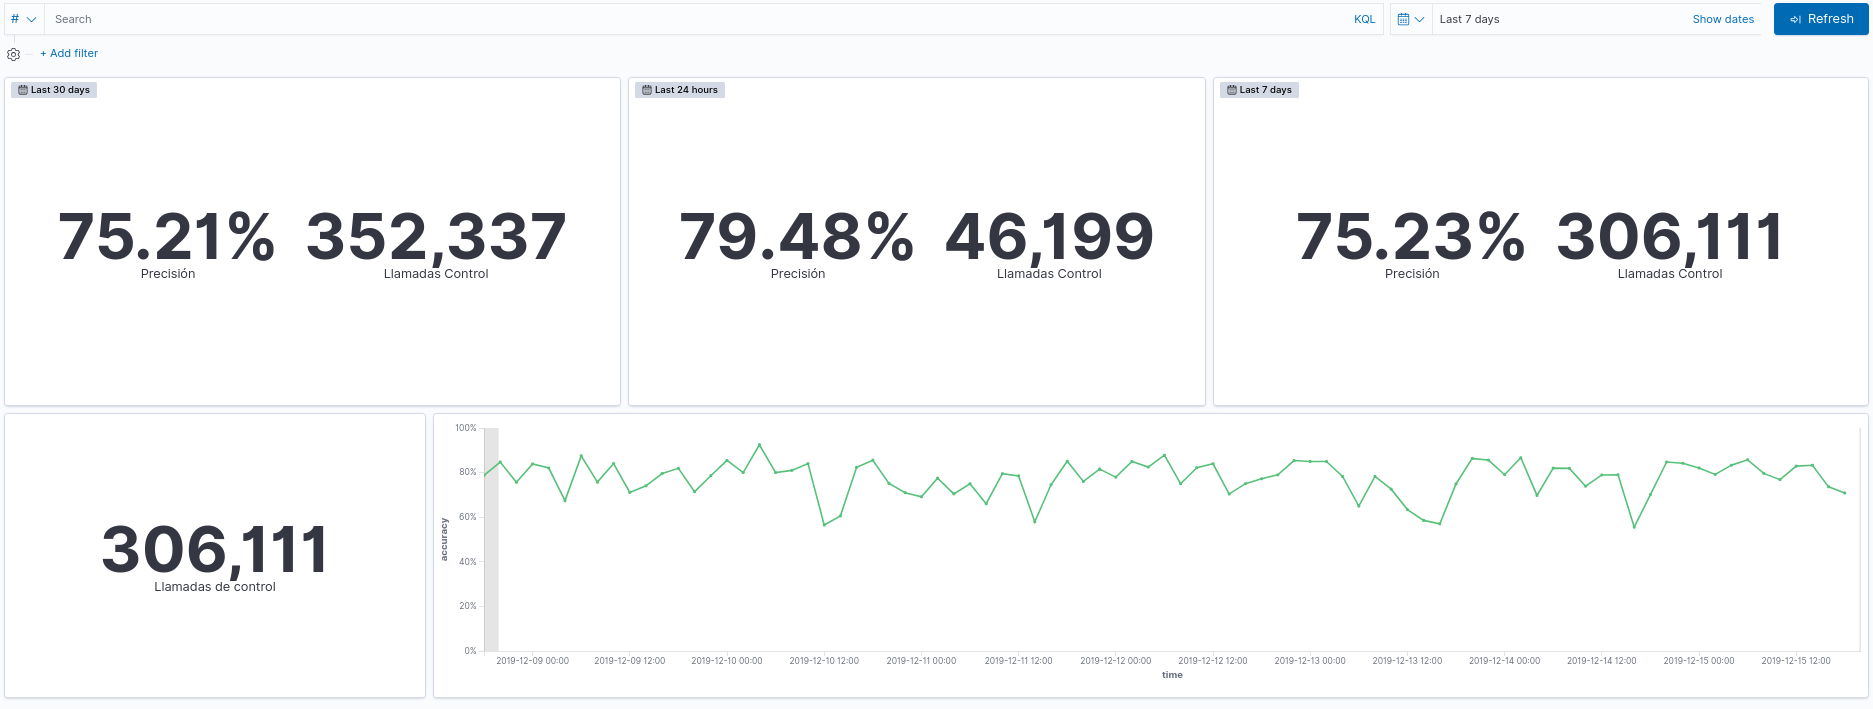
\includegraphics[width=1\textwidth]{images/mant/cmeficiencia}
	\caption{Cuadro de mando eficiencia}
	\label{fig:cmeficiencia}
\end{figure}

Para ello, hemos creado un cuadro de mando que nos permite observar la eficiencia del modelo a lo largo del tiempo. Podemos observarlo en la figura \ref{fig:cmeficiencia}, en él vemos para distintos periodos de tiempo (último mes, último día y última semana), cómo se comporta la precisión de nuestro modelo en función de las llamadas de control recibidas. Además vemos una gráfica con la evolución de la misma para el periodo temporal deseado. Actualmente la precisión se mantiene constante, pero es algo que podría variar a lo largo del tiempo.

La información del cuadro de mando puede consultarse de manera pro-activa o podríamos crear alarmas para reaccionar de una manera reactiva. 


Otra opción que nos permite la capa de servicio creada es investigar las llamadas que hayan sido etiquetadas erróneamente para verificar si, efectivamente, se ha producido un error en la predicción.


\begin{figure}[!ht]
	\centering
	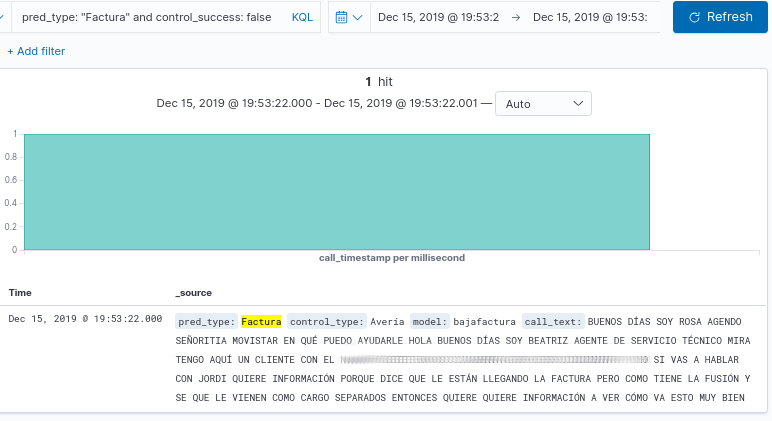
\includegraphics[width=1\textwidth]{images/mant/cm-error.png}
	\caption{\textit{Discover} predicción errónea}
	\label{fig:cm-error}
\end{figure}

En la figura \ref{fig:cm-error} podemos ver un ejemplo de este caso. En la parte superior, vemos como filtramos por llamadas que hayan sido clasificadas como ``Factura'', pero que no hayamos realizado una predicción correcta. En este caso podemos ver que aunque la clase de control sea ``Avería'', el texto de la llamada sí esta tratando un tema de una ``Factura''.  Este tipo de casos ponen de manifiesto que nuestro sistema esta clasificando bien las llamadas, en algunas ocasiones, aunque la etiqueta de control diga lo contrario. Además nos lleva a, en siguientes iteraciones, buscar etiquetas de mayor calidad.

Además de la información presentada, disponemos de otros cuadros de mando, como ya vimos en el capítulo \ref{chapter:servicio} dedicado a la capa de servicio, que nos darán un \textit{feedback} continuo de nuestro sistema.


\section{Integración y despliegue continuos}
\label{section:mant:cicd}

Aunque se trata de un proyecto desarrollado de manera individual y en un único entorno, hemos querido simular lo que sería un flujo de integración y despliegue continuos.

Nuestro objetivo es que cuando realicemos un \textit{push} en la rama \textit{master} de nuestro repositorio de código, se inicie el compilado del mismo de manera automática junto con un conjunto de pruebas unitarias que verifiquen el funcionamiento de cada uno de los servicios. Una vez creado el fichero binario, se enviará a Openshift para que, a partir del mecanismo S2I visto en la sesión \ref{section:cont:s2i}, despliegue de manera automática nuestros servicios.

El servidor de automatización que nos permitirá orquestar todo este flujo será \textit{Jenkins}. \textit{Jenkins} será accionado mediante un \textit{webhook} cada vez se realice un cambio en la rama \textit{master} de nuestro repositorio de \textit{Bitbucket} y a partir de entonces ejecutará el \textit{pipeline} definido.

A continuación mostramos el \textit{pipeline} de Jenkins necesario para la integración y despliegue continuo de los servicios construidos con \textit{K-streams}, para el modelo \textit{tensorflow serving} no lo mostramos ya que es bastante similar excepto por la etapa de compilación.

\vspace{0.5cm}
\begin{minted}[
 	gobble=0,
 	frame=single,
 	linenos]{groovy}
pipeline {
    agent any
    environment {
        BRANCH="master"        
   		PATH = "$PATH:$OC_PATH" 
   		APP_NAME="topicmodel"
		APP_VERSION="1.0-SNAPSHOT-jar-with-dependencies"
   		OPENSHIFT_PROJECT="nbia-prod"
		OPENSHIFT_URL = 'https://openshift'
    }
    stages {
        stage('Checkout') {
            steps {
                git url: 'http://bitbucket/scm/TFM/calls-streams.git', branch: "${BRANCH}", credentialsId: 'bbAdmin'
            }
        }
        stage('Tests') {
            steps {
                withMaven(jdk: 'Java1.8', maven: 'Maven-3.6.0', mavenSettingsConfig: 'nexus') {
                    sh 'mvn test'
                }
            }
        }
        stage('Build') {
            steps {
                withMaven(jdk: 'Java1.8', maven: 'Maven-3.6.0', mavenSettingsConfig: 'nexus') {
                    sh '''
                        ls -lrt;
                        mvn clean package -Dmaven.test.skip=true
                        ls -lrt */*;
                    '''
                }
            }
        }
        stage('Login OpenShift') {
            steps {
                script {
               		withCredentials([[$class: 'UsernamePasswordMultiBinding', credentialsId: 'ocp-t152098', usernameVariable: 'OPENSHIFT_NGBI_USERNAME', passwordVariable: 'OPENSHIFT_NGBI_PASSWORD']]) {
                    	sh 'oc login $OPENSHIFT_URL --username=${OPENSHIFT_NGBI_USERNAME} --password=${OPENSHIFT_NGBI_PASSWORD} -n "${OPENSHIFT_PROJECT}"'
               		}
                }
			}
        } 
        stage('Build Docker Image') {
            steps {
                script {
					try {
						withCredentials([[$class: 'UsernamePasswordMultiBinding', credentialsId: 'ocp-tfm', usernameVariable: 'OPENSHIFT_NGBI_USERNAME', passwordVariable: 'OPENSHIFT_NGBI_PASSWORD']]) {
							sh 'oc start-build topic-model-streaming --from-file=./target/$APP_NAME-$APP_VERSION.jar  --follow -n "${OPENSHIFT_PROJECT}"'  
						}
					} catch (err) {
						echo "Error al delpoy imagen"
						throw new Exception("Error on image deploy")
					}
                }
			}
        } 
    }
    post {
        always {
          step([$class: 'Mailer',
            notifyEveryUnstableBuild: true,
            recipients: "manuel.gomezmontero@telefonica.com",
            sendToIndividuals: true])
        }
    }
}
\end{minted}


En el \textit{pipeline}  podemos ver que en primer lugar definimos las variables de entorno y, posteriormente, tenemos una serie de pasos que comentaremos a continuación:

\begin{itemize}
\item \textit{\textbf{Checkout}} (línea 12): En esta etapa traemos los datos del repositorio \textit{Bitbucket}. 

\item \textit{\textbf{Tests}} (línea 17): En esta etapa se realizan las pruebas unitarias sobre nuestro código.

\item \textit{\textbf{Build}} (línea 24): Realizamos la compilación de nuestro proyecto (omitimos los tests) realizados anteriormente.

\item \textit{\textbf{Login Openshift}} (línea 35): Nos logamos en la plataforma Openshift.

\item \textit{\textbf{Build Docker Image}} (línea 44): Construimos la imagen \textit{docker} con nuestra aplicación.

\item \textit{\textbf{Post}} (línea 59): Una vez hemos finalizado el \textit{pipeline}, enviamos un \textit{mail} informando del estado del mismo. 
 
\end{itemize}


\begin{figure}[!ht]
	\centering
	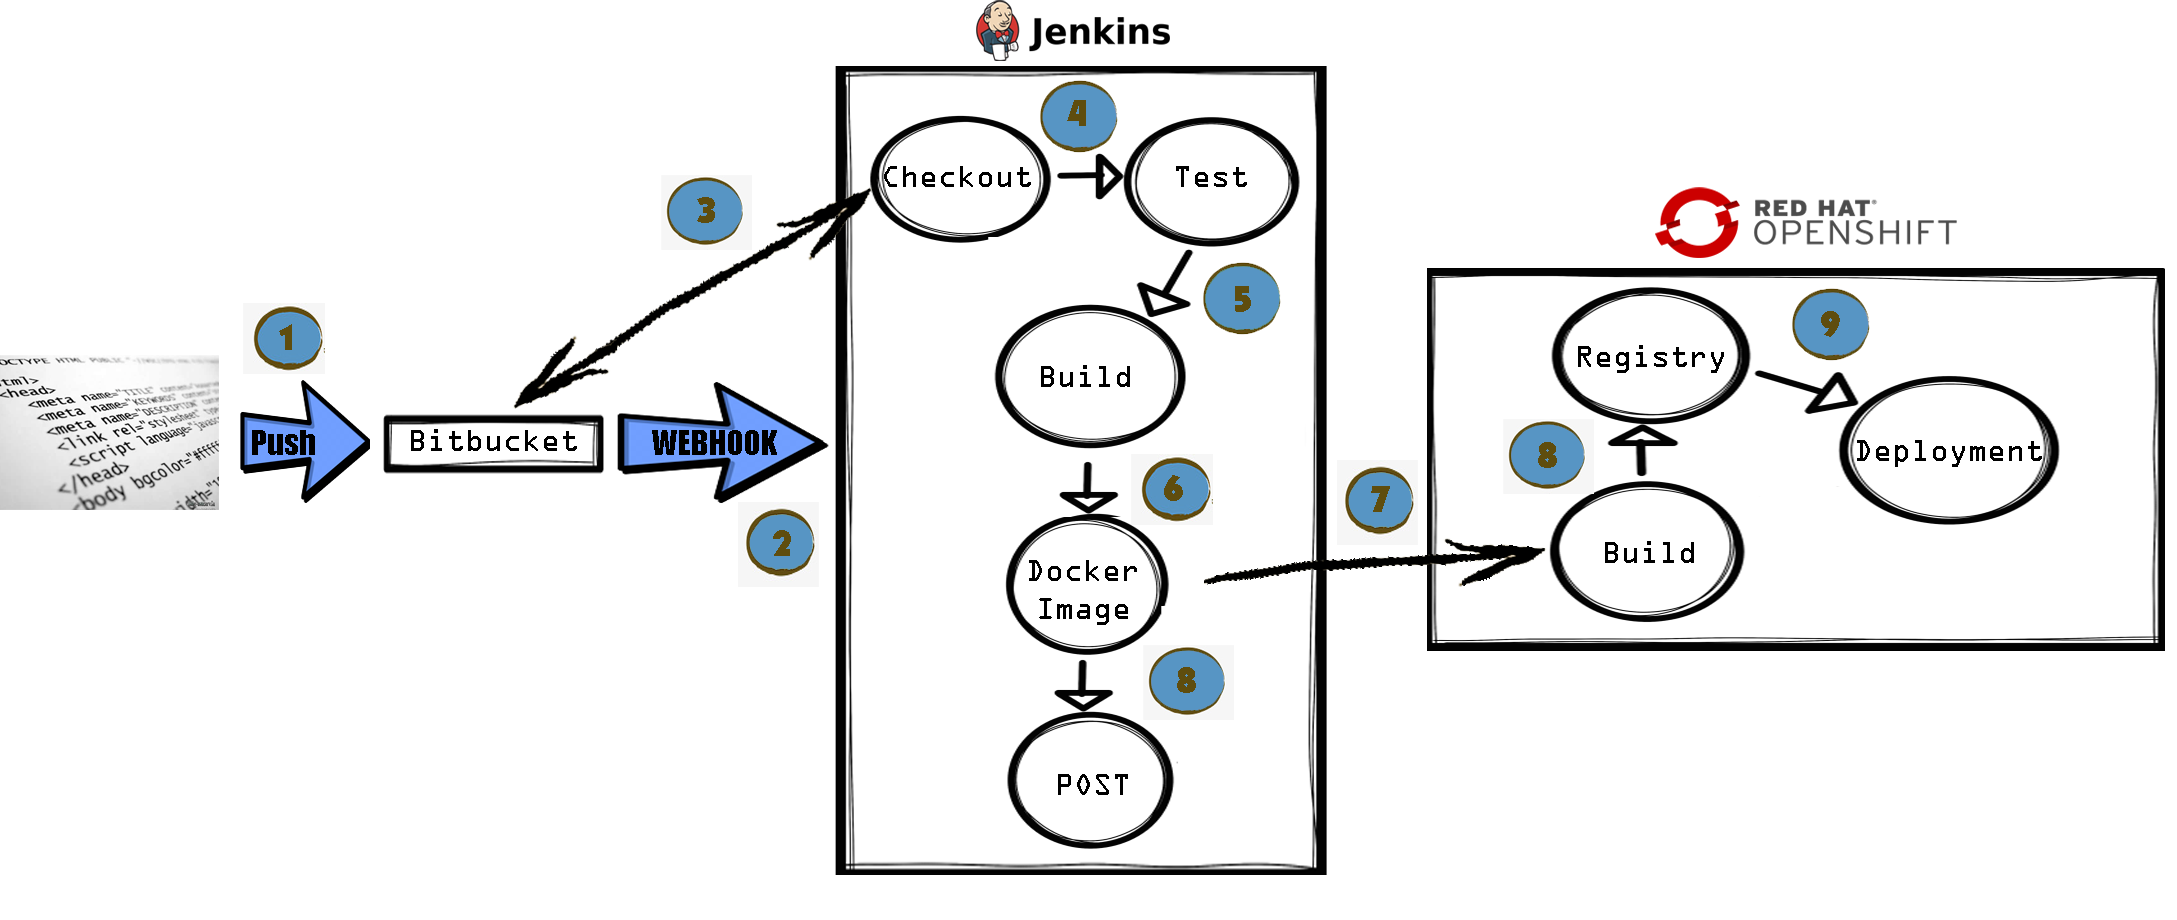
\includegraphics[width=1\textwidth]{images/mant/cicd_v1.png}
	\caption{Despliegue tras \textit{push}}
	\label{fig:flujocicd}
\end{figure}

En la figura \ref{fig:flujocicd} podemos ver cómo sería el flujo completo desde que hacemos un \textit{push} a la rama \textit{master} hasta el despliegue definitivo en producción, con los siguientes pasos:  

\begin{enumerate}
\item El usuario realiza el \textit{push} en el repositorio de Bitbucket en la rama \textit{master}.

\item Se activa un \textit{webhook} que realiza una llamada a \textit{jenkins} para que inicie el \textit{pipeline}. 

\item Jenkins descarga el código de Bitbucket. 

\item Si la fase anterior a finalizado con éxito. Jenkins realiza las pruebas unitarias definidas en el código subido. 

\item Si se superan los tests de la fase anterior Jenkins compila el código fuente para obtener un binario.


\item Una vez obtenido el binario, Jenkins realiza se autentica en la plataforma de Openshift y envía el binario para iniciar un nuevo \textit{build}. 

\item Jenkins espera hasta que el \textit{build} finalice con éxito por parte de Openshift.

\item En este punto el flujo se bifurca tras un \textit{build} satisfactorio:  
	\begin{enumerate}
		\item Openshift registra la nueva imagen de aplicación creada en el \textit{registry} de la plataforma.

		\item Jenkins inicia las acciones \textit{post} del \textit{pipeline}. En nuestro caso, enviar un e-mail (en caso de error este e-mail se enviaría igualmente interrumpiendo el flujo). 
	\end{enumerate}

\item Al actualizarse la imagen la configuración de despliegue de Openshift inicia un nuevo despliegue. Al finalizar con éxito tendríamos operativa la aplicación con nuestro código.

\end{enumerate}

\begin{figure}[!ht]
	\centering
	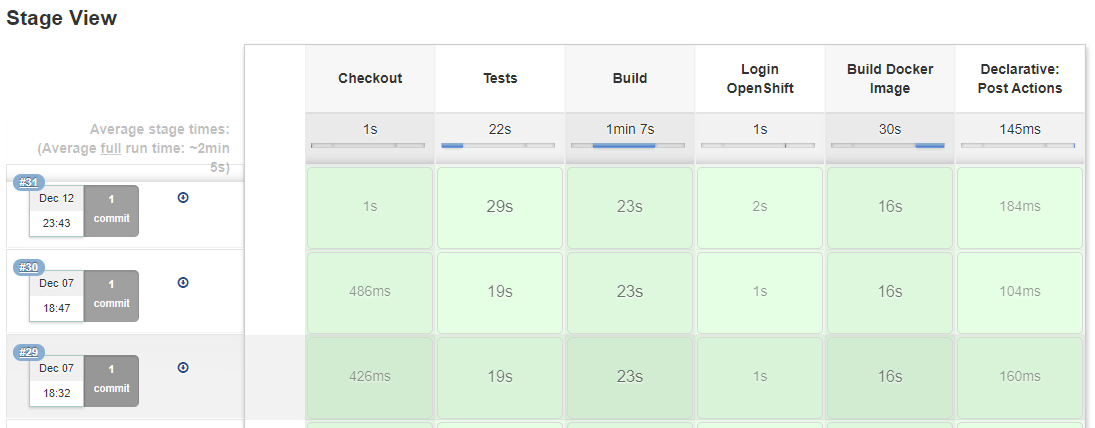
\includegraphics[width=1\textwidth]{images/mant/jenkins-stages}
	\caption{\textit{stages} en Jenkins}
	\label{fig:jenkins}
\end{figure}


 

\begin{figure}[!ht]
	\centering
	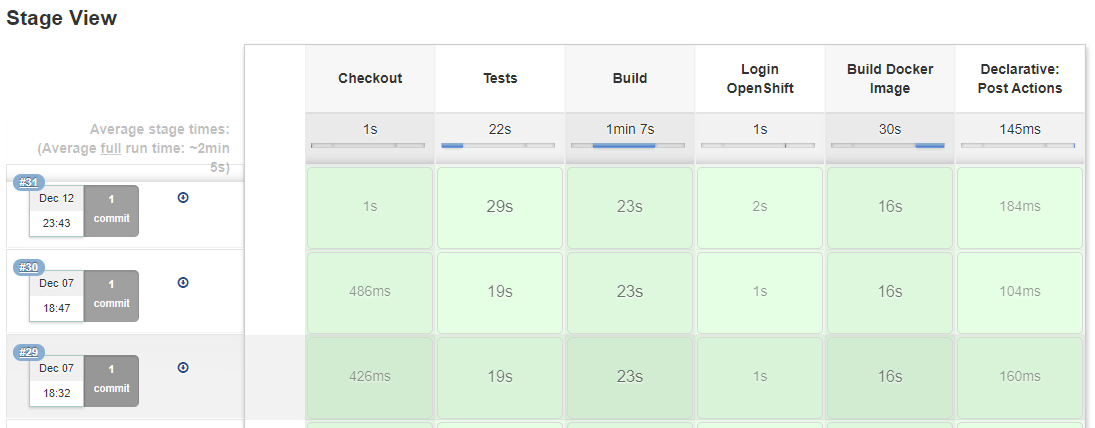
\includegraphics[width=1\textwidth]{images/mant/jenkins-stages}
	\caption{\textit{stages} en Jenkins}
	\label{fig:jenkins}
\end{figure}

El uso de \textit{Jenkins} dentro de este modelo nos proporciona diferentes ventajas más haya de orquestar el proceso que acabamos de comentar. Una de ellas, que podemos observar en la figura \ref{fig:jenkins}, es tener un histórico de todas las compilaciones que se han realizado junto con los \textit{commits} que estaban asociados a las mismas. 


\begin{figure}[!ht]
	\centering
	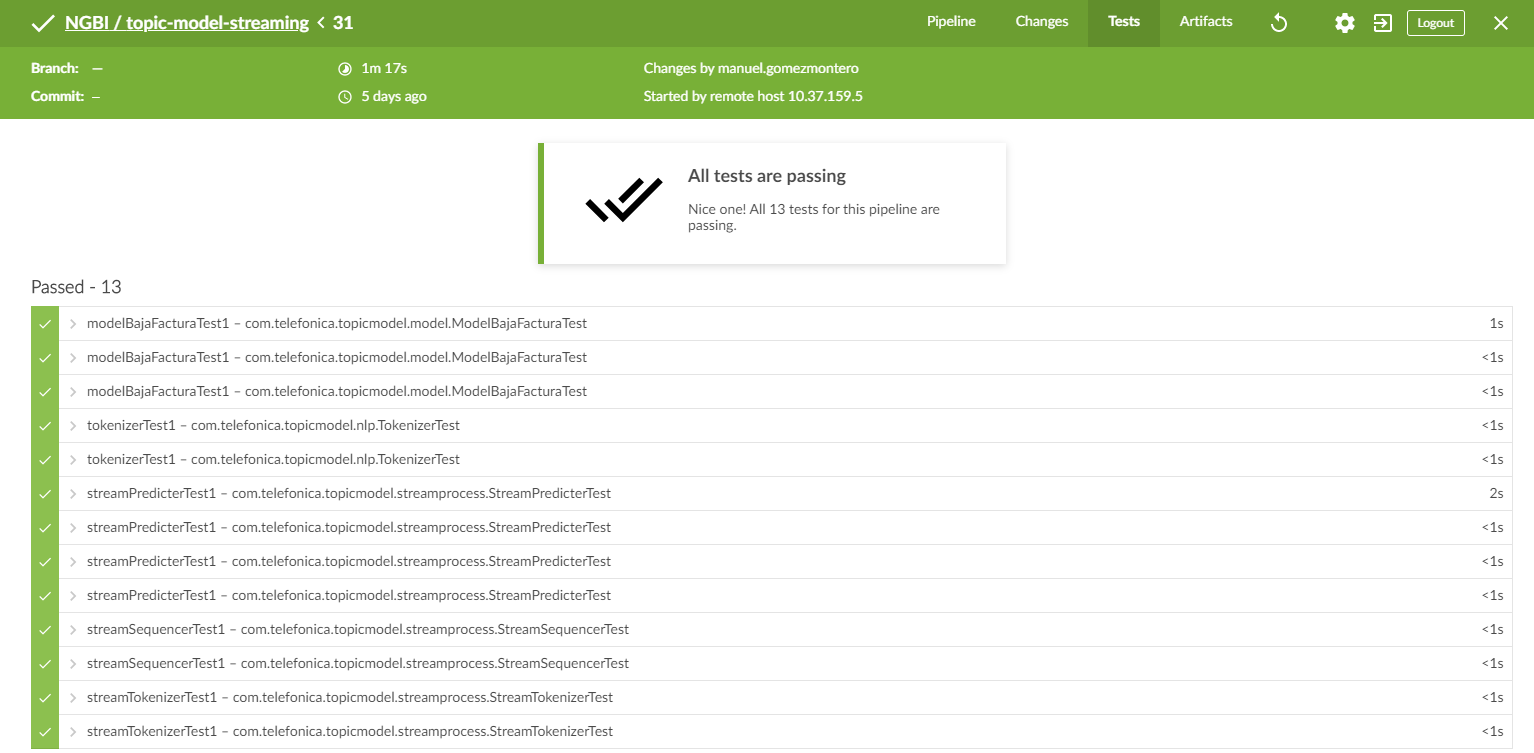
\includegraphics[width=1\textwidth]{images/mant/tests_v2}
	\caption{Resultado de pruebas unitarias}
	\label{fig:jenkins-tests}
\end{figure}

Otra posibilidad es seguir el estado de las diferentes pruebas unitarias que se han realizado en nuestro proyecto, como podemos ver en la figura \ref{fig:jenkins-tests}.
